\documentclass{beamer}
%\usetheme{Singapore}
\usepackage{tikz}
\usetikzlibrary{arrows,automata}

%\usepackage{pstricks,pst-node,pst-tree}
\usepackage{amssymb,latexsym}
\usepackage{graphicx}
\usepackage{fancyvrb}
\usepackage{hyperref}

\newcommand{\bi}{\begin{itemize}}
\newcommand{\ii}{\item}
\newcommand{\ei}{\end{itemize}}
\newcommand{\Show}[1]{\psshadowbox{#1}}


\newcommand{\grf}[2]{\centerline{\includegraphics[width=#1\textwidth]{#2}}}
\newcommand{\tw}{\textwidth}
\newcommand{\bc}{\begin{columns}}
\newcommand{\ec}{\end{columns}}
\newcommand{\cc}[1]{\column{#1\textwidth}}

\newcommand{\bfr}[1]{\begin{frame}[fragile]\frametitle{{ #1 }}}
\newcommand{\efr}{\end{frame}}

\newcommand{\cola}[1]{\begin{columns}\begin{column}{#1\textwidth}}
\newcommand{\colb}[1]{\end{column}\begin{column}{#1\textwidth}}
\newcommand{\colc}{\end{column}\end{columns}}

\title{Introduction to Theory of Computation}
\author{Chapter 4, Turing Machines}

\RecustomVerbatimEnvironment{Verbatim}{Verbatim}{frame=single}

\newcommand{\pth}[5]{\path (#1) edge node {$\frac{#2}{#3 #4}$} (#5); }
\newcommand{\pthl}[5]{\path (#1) edge [bend left] node {$\frac{#2}{#3 #4}$} (#5); }
\newcommand{\pthr}[5]{\path (#1) edge [bend right] node {$\frac{#2}{#3 #4}$} (#5); }
\newcommand{\pthla}[5]{\path (#1) edge [loop above] node {$\frac{#2}{#3 #4}$} (#5); }
\newcommand{\pthlb}[5]{\path (#1) edge [loop below] node {$\frac{#2}{#3 #4}$} (#5); }
\newcommand{\pthlr}[5]{\path (#1) edge [loop right] node {$\frac{#2}{#3 #4}$} (#5); }
\newcommand{\pthll}[5]{\path (#1) edge [loop left] node {$\frac{#2}{#3 #4}$} (#5); }


\begin{document}
\begin{frame}
\maketitle

\end{frame}

\bfr{Even Palindromes}
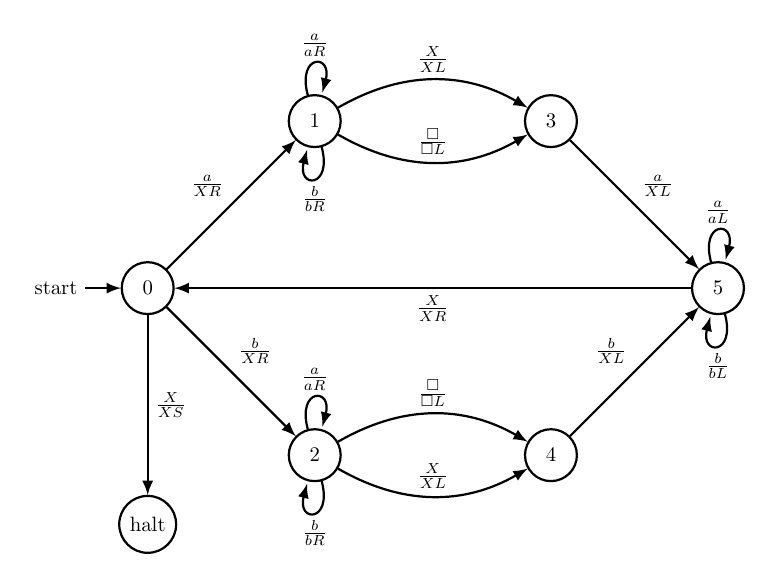
\begin{tikzpicture}[->,>=latex,thick,node distance=4cm,auto,every node/.style={scale=0.75}]
  \node[state,initial] (0) {0};
  \node[state] (1) [above right of=0] {1};
  \node[state] (2) [below right of=0] {2};
  \node[state] (3) [right of=1] {3};
  \node[state] (4) [right of=2] {4};
  \node[state] (5) [below right of=3] {5};
  \node[state] (halt) [below of=0] {halt};
  \path (0) edge node {$\frac{a}{X R}$} (1);
  \path (0) edge node {$\frac{b}{X R}$} (2);
  \path (0) edge node {$\frac{X}{X S}$} (halt);
  \path (1) edge [loop above] node {$\frac{a}{aR}$} (1);
  \path (1) edge [loop below] node {$\frac{b}{bR}$} (1);
  \path (1) edge [bend right] node {$\frac{\square}{\square L}$} (3);
  \path (1) edge [bend left] node {$\frac{X}{X L}$} (3);
  \path (3) edge node {$\frac{a}{X L}$} (5);
  \pthla 2aaR2
  \pthlb 2bbR2
  \pthl 2\square\square L4
  \pthr 2XXL4
  \pth 4bXL5
  \pthla 5aaL5
  \pthlb 5bbL5
  \pth 5XXR0
\end{tikzpicture}

\end{frame}

\bfr{$a^nb^nc^n$}
\begin{tikzpicture}[->,>=latex,thick,node distance=4cm,auto,every node/.style={scale=0.75}]
  \node[state,initial] (0) {0};
  \node[state] (3) [right of=0] {3};
  \node[state] (1) [above of=3] {1};
  \node[state] (2) [right of=1] {2};
  \node[state] (4) [right of=halt] {4};
  \node[state] (halt) [below of=0] {halt};
  \pth 0aXR1
  \pthla 0YYR0
  \pth 0ZZR4
  \pth 0\square\square S{halt}
  \path (1) edge [loop above] node {$\frac{a}{aR}$,$\frac{Y}{YR}$} (1);
  \pth 1bYR2
  \pth 2cZL3
  \path (2) edge [loop above] node {$\frac{b}{bR}$,$\frac{Z}{ZR}$} (2);
  \path (3) edge [loop right] node {$\frac{a}{aL}$,$\frac{b}{bL}$,$\frac{Y}{YL}$,$\frac{Z}{ZL}$} (3);
  \pth 3XXR0
  \pthlr 4ZZR4
  \pth 4\square\square S{halt}
\end{tikzpicture}

\end{frame}

\bfr{Equivalent models:}
\begin{enumerate}
\item One-tape Turing machines.
\item $k$-tape Turing machines.
\item Non-deterministic Turing machines.
\item Java programs.
\item Scheme programs.
\item C++ programs.
\item ...
\end{enumerate}
\end{frame}

\bfr{The Church-Turing Thesis}

{\Large \bf
  Every computational process that is intuitively considered to
  be an algorithm can be converted to a Turing machine.  }
\end{frame}

\bfr{Decidability}

A language $A$ over $\Sigma$
is {\em decidable} if there exists a Turing machine $M$
such that for every string $w\in\Sigma^*$:
\begin{enumerate}
\item If $w\in A$ then $M$, started on $w$, halts in the accept state.
\item If $w\not\in A$ then $M$, started on $w$, halts in the reject state.
\end{enumerate}
\end{frame}

\bfr{Describing machines and problems as strings}
\begin{itemize}
\item We assume any machine (DFA, PDA, TM) can be described by a
  string $M$ using some alphabet.
\item The input to any machine is a string $w$ using some alphabet.
\item We can thus describe both a machine $M$ and its input $w$, with a
  pair of strings: $( M,w )$.
\item This pair can be converted to  a single string
  $\langle M,w  \rangle$.
\item  For convenience, we assume   $\langle M,w  \rangle$ is
  encoded in binary.
  \item In general, $\langle M\rangle$ means: encode $M$ as a binary
    string. 
\item We can now define a language $A$ as the set of all strings
  $\langle M,w \rangle$ such that $w$ is in the computation model of
  $M$. 
\end{itemize}
\end{frame}

\bfr{The language $A_{DFA}$ is decidable}
\[
A_{DFA} = \{ \langle M,w\rangle : \mbox{$M$ is a DFA that accepts $w$}\}
\]

Proof?

\pause

\begin{itemize}
\item Given input $\langle M,w\rangle$:
  \begin{itemize}
  \item Run $M$ on $w$.
  \item It must terminate.
  \item If it accepts, accept, else reject.
  \end{itemize}
\end{itemize}
\end{frame}

\bfr{The language $A_{NFA}$ is decidable}
\[
A_{NFA} = \{ \langle M,w\rangle : \mbox{$M$ is a NFA that accepts $w$}\}
\]


Proof?

\pause

\begin{itemize}
\item Given input $\langle M,w\rangle$:
  \begin{itemize}
  \item Convert NFA $M$ to DFA $N$.
  \item This algorithm terminates.
  \item Run $N$ on $w$.
  \item It must terminate.
  \item If it accepts, accept, else reject.
  \end{itemize}
\end{itemize}
\end{frame}

\bfr{The language $A_{CGF}$ is decidable}
\[
A_{NFA} = \{ \langle M,w\rangle : \mbox{$M$ is a CFG that accepts $w$}\}
\]


Proof?

\pause

\begin{itemize}
\item Given input $\langle M,w\rangle$:
  \begin{itemize}
  \item Convert CFG $M$ to Chomsky normal form CFG $N$.
  \item This algorithm terminates.
  \item Run $N$ on $w$ for all derivations up to length $2|w|$.
  \item There are a finite number of these, so it must terminate.
  \item If any derivation accepts, accept, else reject.
  \end{itemize}
\end{itemize}
\end{frame}


\bfr{The language $A_{TM}$ is not decidable.}
\[
A_{TM} = \{ \langle M,w\rangle : \mbox{$M$ is a TM that accepts $w$}\}
\]

Proof?\pause\ By contradiction. 

\begin{itemize}
  \item Assume there is a TM $H$ that decides this
    language.
  \item Construct the following TM, $D$:
    
\centerline{
  \fbox{
    \parbox{3in}{
      $D$: On input $\langle M\rangle$:
      \begin{description}
      \item[Step 1:] Run $H$ on $\langle M, \langle M \rangle\rangle$.
      \item[Step 2:] If $H$ accepts, reject, else accept.
      \end{description}
    }
  }
}
\item If $H$ accepts $\langle D, \langle D \rangle\rangle$, then
  $D$ rejects $\langle D \rangle$.
\item If $H$ rejects $\langle D, \langle D \rangle\rangle$, then
  $D$ accepts $\langle D \rangle$.
\item $H$ does not recognize $A_{TM}$.
\end{itemize}

\end{frame}

\bfr{Diagonal argument}
\begin{itemize}
  \item
    Machine $H$ that decides $A_{TM}$ can fill in this table:

\fbox{\parbox{4in}{\[
\begin{array}{cccccccc}
 &  \langle M_0 \rangle &  \langle M_1 \rangle &  \langle M_2 \rangle
 &  \langle M_3 \rangle &  \langle M_4 \rangle &  \langle M_5 \rangle
  & ...\\
  M_0 & \bf accept & accept & accept & reject & accept & reject & ...\\
  M_1 & accept & \bf reject & accept & accept & accept & reject & ...\\
  M_2 & accept & reject & \bf accept & accept & accept & reject & ...\\
  M_3 & accept & accept & reject & \bf reject & accept & accept & ...\\
  M_4 & reject & accept & accept & reject & \bf accept & accept & ...\\
  M_5 & reject & reject & accept & accept & accept & \bf reject & ...\\
  ... &  ... &  ... &  ... &  ... &  ... &  ... &  ... 
\end{array}
\]}}

\item
Machine $D$ uses $H$ to give the opposite answer on the diagonal.
\item
  Machine $H$ must give the wrong answer somewhere on machine $D$.
  \end{itemize}
\end{frame}



\bfr{The language $Halt$ is not decidable.}
\[
Halt = \{ \langle M,w\rangle : \mbox{$M$ is a TM that terminates on $w$}\}
\]

Proof?\pause

By contradiction.  Assume there is a TM $H$ that decides this
language.  Construct the following TM, $Q$:

\centerline{
  \fbox{
    \parbox{3in}{
      $Q$: On input $\langle M\rangle$:
      \begin{description}
      \item While $H(\langle M,\langle M \rangle \rangle)$ do endwhile
      \end{description}
    }
  }
}

\begin{itemize}
\item
  What happens if we run $Q$ on itself?
\item
  $Q(\langle Q\rangle) $
terminates iff   $Q(\langle Q\rangle) $ does not terminate.
\end{itemize}
\end{frame}

\bfr{Rice's Theorem}
Let $\mathcal{T}$ be the set of all binary encoded TMs.

Let $\mathcal{P}$ be a subset of $\mathcal{T}$ such that
\begin{enumerate}
\item $\mathcal{P}\not=\emptyset$
\item $\mathcal{P}\not=\mathcal{T}$
\item If $L(M_1) = L(M_2)$, then either both or neither is in $\mathcal{P}$.
\end{enumerate}
Then $\mathcal{P}$ is undecidable.
\end{frame}

\bfr{Enumerability}

A language $A$ over $\Sigma$
is {\em enumerable} if there exists a Turing machine $M$
such that for every string $w\in\Sigma^*$:
\begin{enumerate}
\item If $w\in A$ then $M$, started on $w$, halts in the accept state.
\item If $w\not\in A$ then $M$, started on $w$, either halts in the
  reject state or loops forever.
\end{enumerate}
\end{frame}

\bfr{Hilbert's problem is enumerable but not decidable}
\begin{eqnarray*}
Hilbert = \{\langle p \rangle &:& \mbox{$p$ is a polynomial with integer
  coefficients}\\ &&\mbox{that has an integral root}\}
\end{eqnarray*}
\end{frame}


\bfr{The language $A_{TM}$ is enumerable but not decidable.}
\[
A_{TM} = \{ \langle M,w\rangle : \mbox{$M$ is a TM that accepts $w$}\}
\]

Proof?
\end{frame}

\bfr{Why do we call it enumerable?}
\begin{itemize}
\item If we can enumerate the elements with an algorithm, then we can
  create an algorithm to correctly identify elements of the set.
  \item If we can correctly identify elements of the set, then we can
    build an algorithm to enumerate them.
\end{itemize}
\end{frame}

\bfr{Busy beavers are not enumerable}
The $n$th busy beaver number is the largest (finite) number of 1s that
can be output by a Turing machine with $n$ states.
\end{frame}


\bfr{2 State Busy Beaver: four 1s}
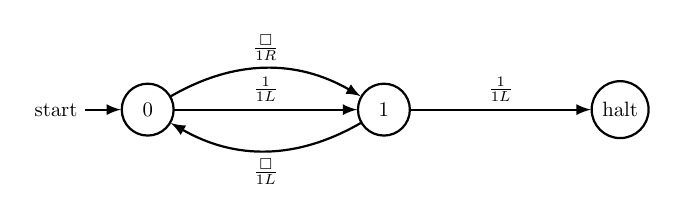
\begin{tikzpicture}[->,>=latex,thick,node distance=4cm,auto,every node/.style={scale=0.75}]
  \node[state,initial] (0) {0};
  \node[state] (1) [right of =0] {1};
  \node[state] (halt) [right of=1] {halt};
  \pthl 0\square 1R1
  \pth 011L1
  \path (1) edge [bend left] node {$\frac{\square}{1L}$} (0);
  \path (1) edge  node {$\frac{1}{1L}$} (halt);
\end{tikzpicture}
 
\end{frame}


\bfr{3 State Busy Beaver: six 1s }
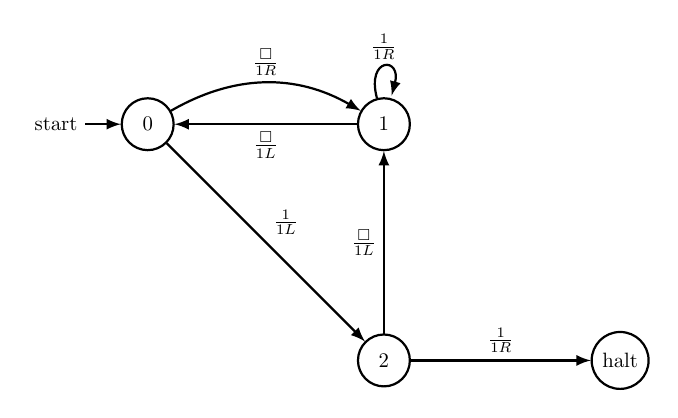
\begin{tikzpicture}[->,>=latex,thick,node distance=4cm,auto,every node/.style={scale=0.75}]
  \node[state,initial] (0) {0};
  \node[state] (1) [right of =0] {1};
  \node[state] (2) [below of =1] {2};
  \node[state] (halt) [right of=2] {halt};
  \pthl 0\square 1R1
  \pth 011L2
  \pth 1\square 1L0
  \pthla 111R1
  \pth 2\square 1L1
  \pth 211R{halt}
\end{tikzpicture}
 
\end{frame}

\bfr{4 State Busy Beaver: thirteen 1s}
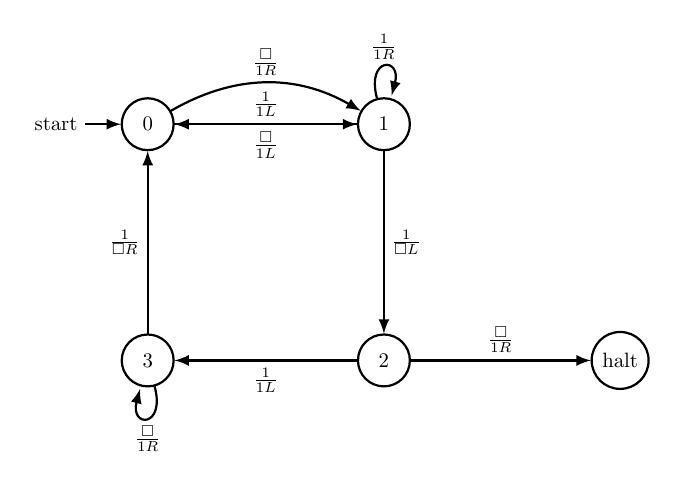
\begin{tikzpicture}[->,>=latex,thick,node distance=4cm,auto,every node/.style={scale=0.75}]
  \node[state,initial] (0) {0};
  \node[state] (1) [right of =0] {1};
  \node[state] (2) [below of =1] {2};
  \node[state] (3) [below of =0] {3};
  \node[state] (halt) [right of=2] {halt};
  \pthl 0\square 1R1
  \pth 011L1
  \pth 1\square 1L0
  \pthla 111R1
  \pth 11\square L2
  \pth 2\square 1R{halt}
  \pth 211L3
  \pthlb 3\square 1R3
  \pth 31\square R0
\end{tikzpicture}
 
\end{frame}


\bfr{5 State Busy Beaver (?): 4098 1s}
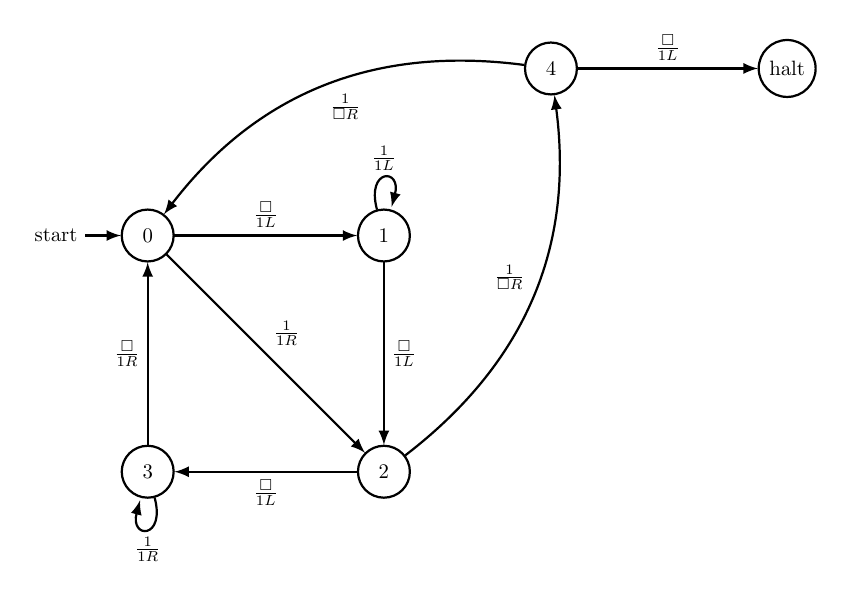
\begin{tikzpicture}[->,>=latex,thick,node distance=4cm,auto,every node/.style={scale=0.75}]
  \node[state,initial] (0) {0};
  \node[state] (1) [right of =0] {1};
  \node[state] (3) [below of =0] {3};
  \node[state] (2) [right of=3] {2};
  \node[state] (4) [above right of=1] {4};
  \node[state] (halt) [right of=4] {halt};
  \pth 0\square 1L1
  \pth 011R2
  \pth 1\square 1L2
  \pthla 111L1
  \pth 2\square 1L3
  \pthr 21\square R4
  \pth 3\square 1R0
  \pthlb 311R3
  \pth 4\square 1L{halt}
  \pthr 41\square R0
\end{tikzpicture}
 
\end{frame}

\bfr{Proof Busy Beaver function is uncomputable}

Proof by contradiction.

\begin{itemize}
\item
Let $bb(n)$ be the largest (finite) number of 1's output by a Turing Machine
with $n$ states.
\item
Suppose there is a Turing Machine $M_{bb}$ that computes $bb(n)$, that is,
starting with $n$ on the tape, the machine halts with $bb(n)$ on the tape.

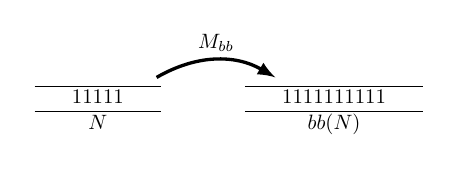
\begin{tikzpicture}[->,>=latex,very thick,node distance=4cm,auto,every node/.style={scale=0.75}]
  \node (1) {
    \begin{tabular}{ccc}\hline
      & 11111 & \\\hline
      & $N$ & \\
    \end{tabular}
  };
  \node (2) [right of=1] {
    \begin{tabular}{ccc}\hline
      & 1111111111 & \\\hline
      & $bb(N)$ & \\
    \end{tabular}
    };
  \path (1) edge [bend left] node {$M_{bb}$} (2);
  \end{tikzpicture}

\item Note: this is a new use of TMs, computing a function
  from input to output, not recognizing a language.
\end{itemize}
\end{frame}

\bfr{Busy Beaver proof}
\begin{itemize}

\item
Let $g(n) = bb(2n)$.  We can build a TM for $g$ by starting with
a machine that doubles the input, and then runs the machine  $M_{bb}$.

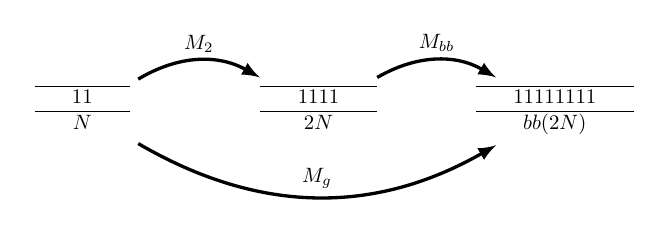
\begin{tikzpicture}[->,>=latex,very thick,node distance=4cm,auto,every node/.style={scale=0.75}]
  \node (3) {
    \begin{tabular}{ccc}\hline
      & 11 & \\\hline
      & $N$ & \\
    \end{tabular}
  };
  \node (4) [right of = 3] {
    \begin{tabular}{ccc}\hline
      & 1111 & \\\hline
      & $2N$ & \\
    \end{tabular}
  };
  \node (5) [right of=4] {
    \begin{tabular}{ccc}\hline
      & 11111111 & \\\hline
      & $bb(2N)$ & \\
    \end{tabular}
    };
  \path (3) edge [bend left] node {$M_{2}$} (4);
  \path (4) edge [bend left] node {$M_{bb}$} (5);
  \path (3) edge [bend right] node {$M_g$} (5);
  \end{tikzpicture}

\item
Suppose the machine for $g$, $M_g$  has $k$ states.

\end{itemize}
\end{frame}

\bfr{Busy Beaver proof}

\begin{itemize}
\item
  Build a machine $M_{2k}$ with $2k$ states that does nothing but put
  $2k$ 1s on a blank tape.
  \item Now build a machine $M_{D}$
  that starts by putting $2k$ 1's on the tape, and then runs the $M_g$
  machine.

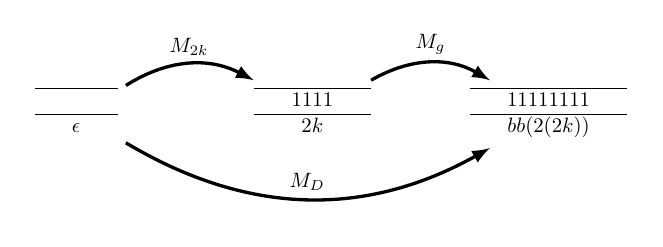
\begin{tikzpicture}[->,>=latex,very thick,node distance=4cm,auto,every node/.style={scale=0.75}]
  \node (6) {
    \begin{tabular}{ccc}\hline
      &  & \\\hline
      & $\epsilon$ & \\
    \end{tabular}
  };
  \node (7) [right of = 6] {
    \begin{tabular}{ccc}\hline
      & 1111 & \\\hline
      & $2k$ & \\
    \end{tabular}
  };
  \node (8) [right of=7] {
    \begin{tabular}{ccc}\hline
      & 11111111 & \\\hline
      & $bb(2(2k))$ & \\
    \end{tabular}
    };
  \path (6) edge [bend left] node {$M_{2k}$} (7);
  \path (7) edge [bend left] node {$M_g$} (8);
  \path (6) edge [bend right] node {$M_{D}$} (8);
  \end{tikzpicture}
\item $M_{D}$ can be built with $3k$ states.
\item The output of $M_{D}$ is $g(2k) = bb(2(2k)) = bb(4k)$ 1s.
\item Do you see the problem?
\end{itemize}
\end{frame}
\end{document}

